%%%%%%%%%%%%%%%%%%%%%%%%%%%%%%%%%%%%%%%%%%%%%%%%%%%%%%%%%%%
%                            Section 5.3
%%%%%%%%%%%%%%%%%%%%%%%%%%%%%%%%%%%%%%%%%%%%%%%%%%%%%%%%%%%
\chapter{5.3 Systems of Inequalities}
%%%%%%%%%%%%%%% SECTION HEADER %%%%%%%%%%%%%%%%
\rhead{3}
\lhead{Systems of Inequalities}
%%%%%%%%%%%%%%%%%%% START %%%$%%%%%%%%%%%%%%%%%
\section{A linear inequality}
A linear inequality in two variables is similar to linear equation in two 
variables. However, instead of $=$ sign we might have one of the following signs 
$<$, $>$, $\leq$ and $\geq$. Therefore, it can be written as
	\begin{align*}
		Ax+By &<C\\
		Ax+By &>C\\
		Ax+By &\leq C\\
		Ax+By &\geq C
	\end{align*}
examples are $x+2y<-3$, \ $4x+y\geq \frac{2}{3}$, \ and \ $\frac{4}{3}
y-2\sqrt{3}\leq 0$.
% ============= SECTION
\section{Graphing a linear inequality}
To graph a linear equality, you first need to find the boundary line. The boundary line is the line that divide the $xy$-plane into two planes. One of the half-plane will be our answer. To find out which sections is our answer, we use a test point within one of them; If it satisfies the inequality, thus that area containing the test point is our solution. Otherwise, the other area is solution.\\
If we have one of these inequalities $\leq$ or $\geq$, it means the boundary line itself is included in our solution. So we use a solid line. If we have other inequalities $<$ or $>$, then the boundary line is not included in our answer. We indicate this using dashed line.\\
For example, consider $x+y>2$. The boundary line is $x+y=2$. This boundary line divide the whole $xy$-plane into two sections. If we choose $(0,0)$ as our test point, we'll see that this test point does not satisfy the inequality
    \[
        0+0>2 \quad \xmark
    \]
Therefore, the half-plane containing $(0,0)$ is not our solution and the other one will be our final solution. The following graph shows the boundary line, correct area (shaded in green), and the wrong area (shaded in red). When solving linear inequality, we only need to shade the correct section.
% ============= Graph ================
\begin{figure}[H]
 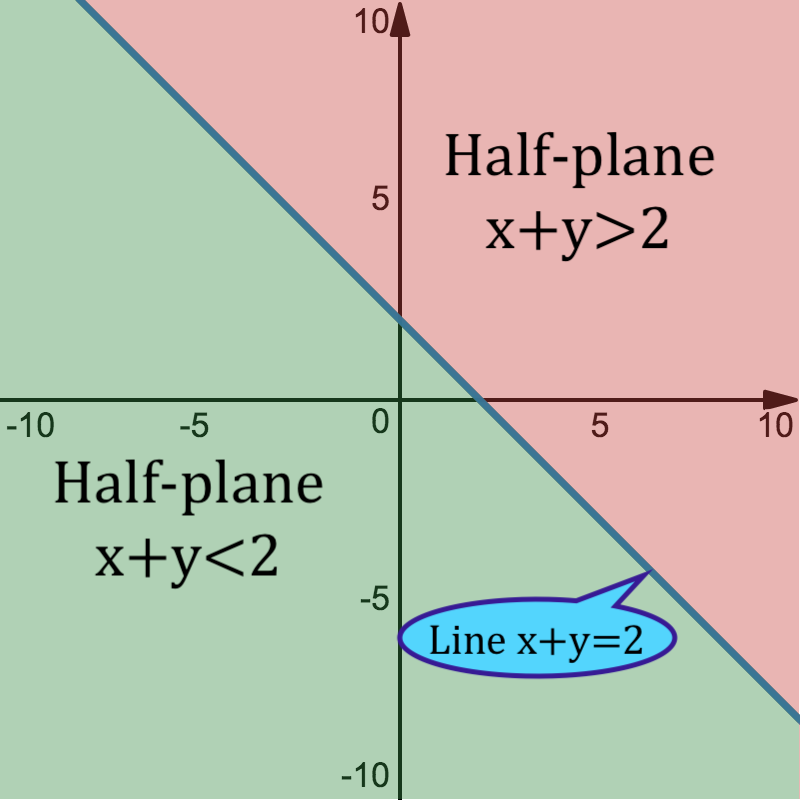
\includegraphics[width=5cm]{pics/line.png}
 \centering
  \caption{The boundary line of $x+y>2$. The correct area is shaded in green}
\end{figure}
% ================================= END
	%
	\begin{tcolorbox}[title=Graphing a linear inequality, 
	                  fonttitle=\bfseries,
	                  colframe=blue!70!red,
	                  colback=white]
	\begin{enumerate}
	    \item Replace the inequality sign with $=$. This equation is our boundary line.
    	\item Draw the boundary line. Draw a dashed line, if the original inequality contains $<$ or $>$. Draw a solid line, if the original inequality contains $\leq$ or $\geq$.
	    \item Choose a test point from one of the half-planes.
    	\item Plug the test point into original inequality.
    	\item If the test point satisfies the inequality, then shade the half-plane contains this point. Otherwise, shade the other half-plane.
	\end{enumerate}
	\end{tcolorbox}
% ========================= EXAMPLE 1
\begin{example}
	 Graph  $y-2x\leq -4$.
\end{example}
%
The boundary line is $y-2x=-4$. Draw the line and since we have $\leq$ sign, therefore make it
solid. Using $(0,0)$ as our test point, we'll see
\begin{align*}
	0-2(0) &\leq -4 \\
	0 &\leq -4 \quad \xmark
\end{align*}
Therefore, we should shade the other half-plane which does not contain $(0,0)$.
%
\begin{figure}[H]
 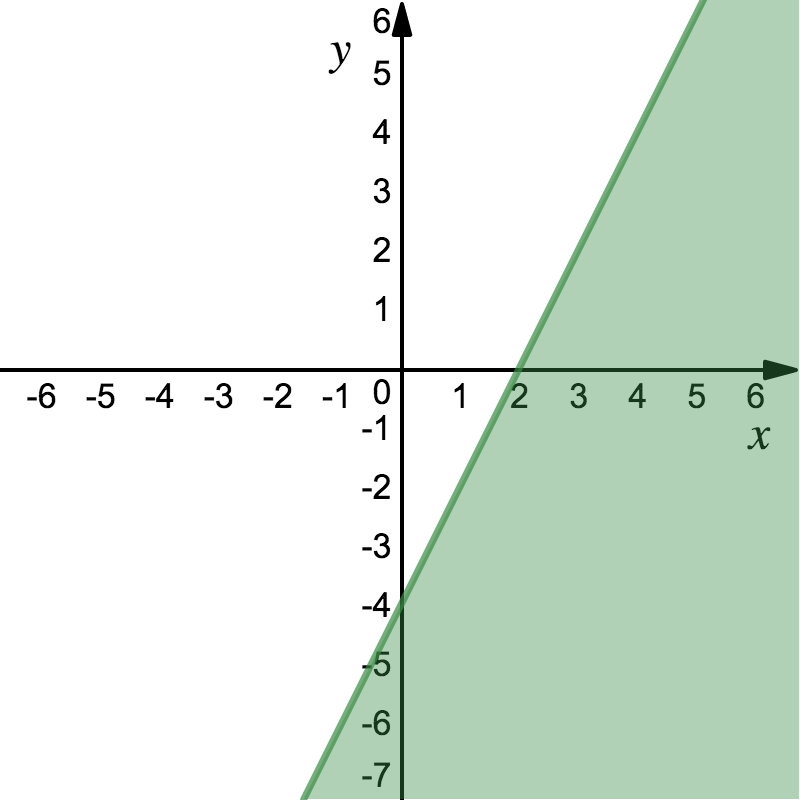
\includegraphics[width=5cm]{pics/pic1.png}
 \centering
  \caption{The graph of $y-2x\leq -4$.}
\end{figure}
% ========================= EXAMPLE 2
\begin{example}
	Graph $y-3x > 1$.
\end{example}
%
Here the boundary line is $y-3x=1$. Draw a dashed line because of $>$ sign. Using $(0,0)$ as our test point, we get
\begin{align*}
	0-3(0) &> 1 \\
	0 &> 1 \quad \xmark
\end{align*}
Therefore, we shade the half-plane not containing the point $(0,0)$.
%
\begin{figure}[H]
 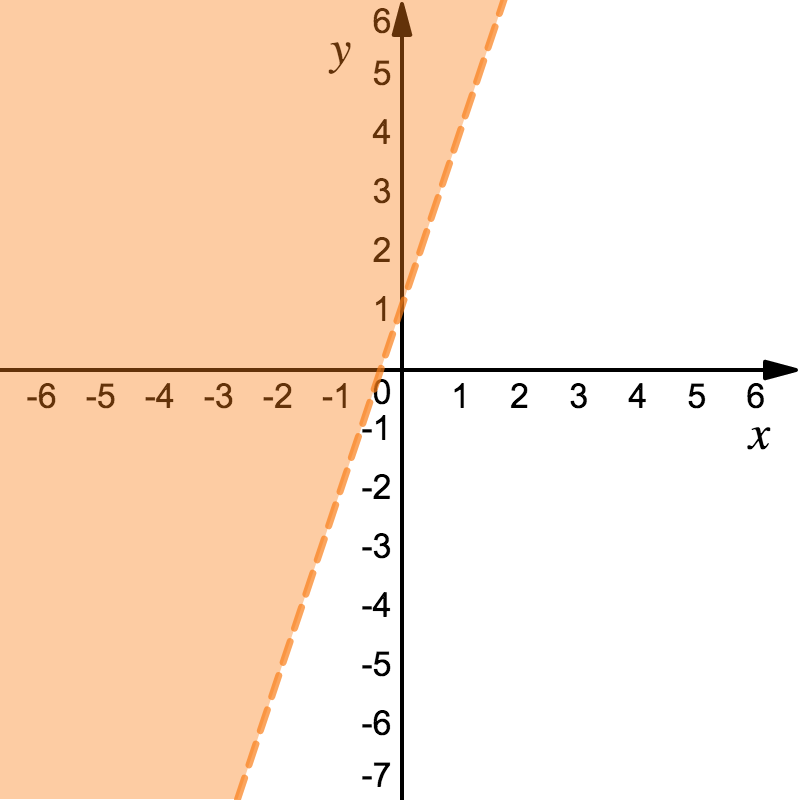
\includegraphics[width=5cm]{pics/pic2.png}
 \centering
  \caption{The graph of $y-3x> 1$.}
\end{figure}
% ================== SECTION
\section{Graphing systems of linear inequalities}
Two linear inequalities create a system of linear inequalities. Our previous work in this chapter dealt with finding the solution set of a system of linear equations. That solution set represented the points of intersection of the graphs of the equations in the system. \\
In this section, we extend that idea to include systems of linear inequalities. In this case, the solution set is all ordered pairs that satisfy each inequality. The graph of the solution set of a system of linear inequalities is then the intersection of the graphs of the individual inequalities.
% ========================= EXAMPLE 3
\begin{example}
	Graph the solution set of the systems:
	\begin{equation*}
		\begin{cases}
			x+y >4 \\
			x-y <2
		\end{cases}
	\end{equation*}
\end{example}
%
The boundary lines of each equation are
	\begin{equation*}
		\begin{cases}
			x+y =4 \\
			x-y =2
		\end{cases}
	\end{equation*}
%
Draw the first one in dashed. Next we will choose $(0,0)$ as a test point.Since (0,0) does not satisfy the inequality, \, $0+0>4\,\,\xmark$ ,and we must shade the region where (0,0) is not included.  That’s why we shade the area above the line.
%
\begin{figure}[H]
 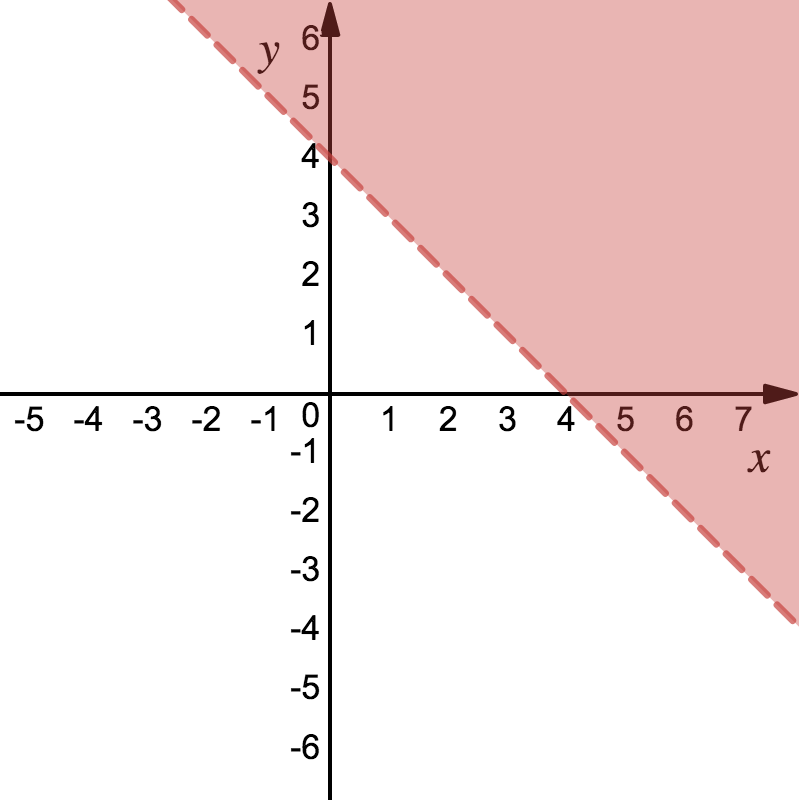
\includegraphics[width=4.5cm]{pics/pic3.png}
 \centering
  \caption{The graph of $x+y>4$.}
\end{figure}
%
Graph the second boundary line, $x-y=2$, use $(0,0)$ as a test point. You'll see this point satisfy the inequality,\, $0-0<2\,\,\checkmark$. So shade the area containing this point. Notice the boundary line is a dashed line because it’s not included in our answer. 
%
\begin{figure}[H]
 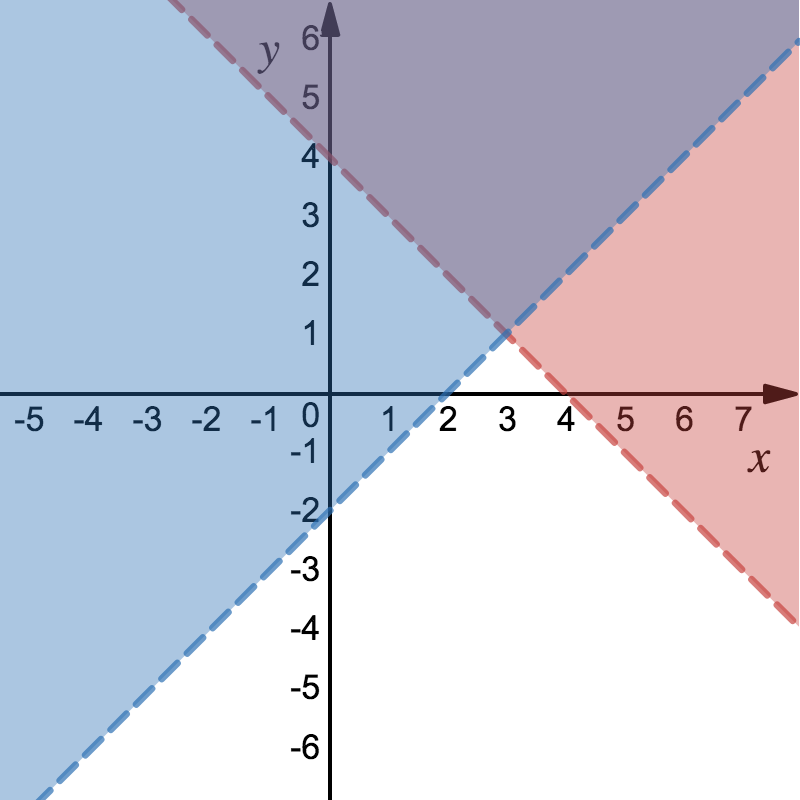
\includegraphics[width=4.5cm]{pics/pic4.png}
 \centering
  \caption{The graph of $x-y<2$ in blue and $x+y>4$ in red.}
\end{figure}
% 
The darker shaded region is the intersection of two graphs. Thus, the solution to the system of two inequality is the darker shaded region and its boundary lines.
% 
\begin{figure}[H]
 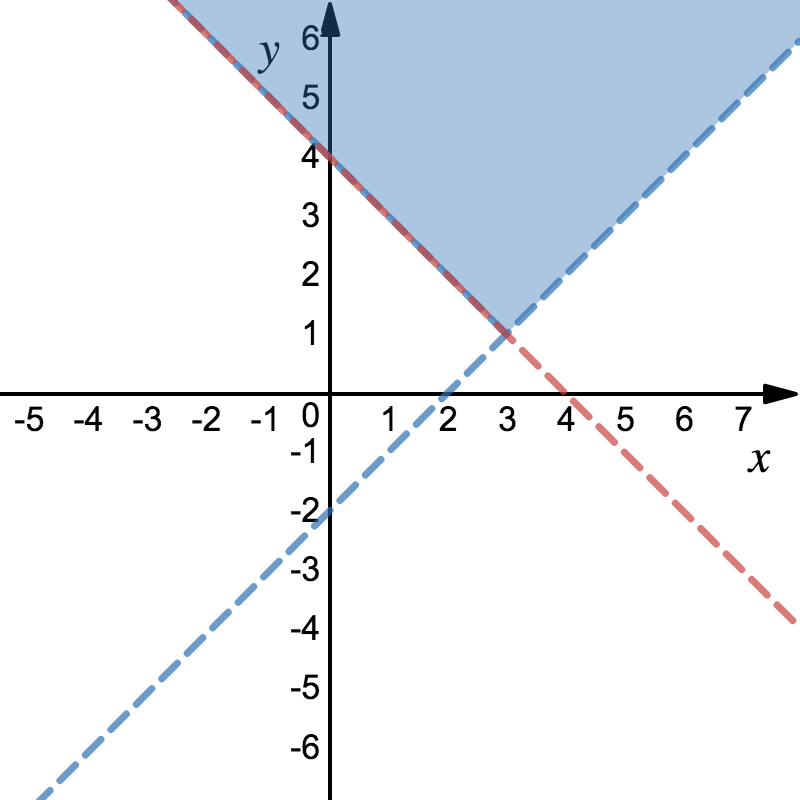
\includegraphics[width=4cm]{pics/pic5.png}
 \centering
  \caption{The graph of $x-y<2$ and $x+y>4$.}
\end{figure}
% ============ NOTE
\begin{note}
	A system of inequalities has no solution if there are no overlapping area. The solution set is $\oslash$.
\end{note}
% ========================= EXAMPLE 4
\begin{example}
	Graph the solution set of the systems:
	\begin{equation*}
		\begin{cases}
			x+y <4 \\
			-2\leq x<1 \\
			y > -3
		\end{cases}
	\end{equation*}
\end{example}
%
The boundary lines of each equation are
	\begin{equation*}
		\begin{cases}
			x+y = 4 \\
			x = -2 \\
			x = 1 \\
			y = -3
		\end{cases}
	\end{equation*}
To graph the first inequality, draw $x+y=4$ in dashed. Because the test point $(0,0)$ satisfies the inequality, we shade the half-planes contains this point.
% 
\begin{figure}[H]
 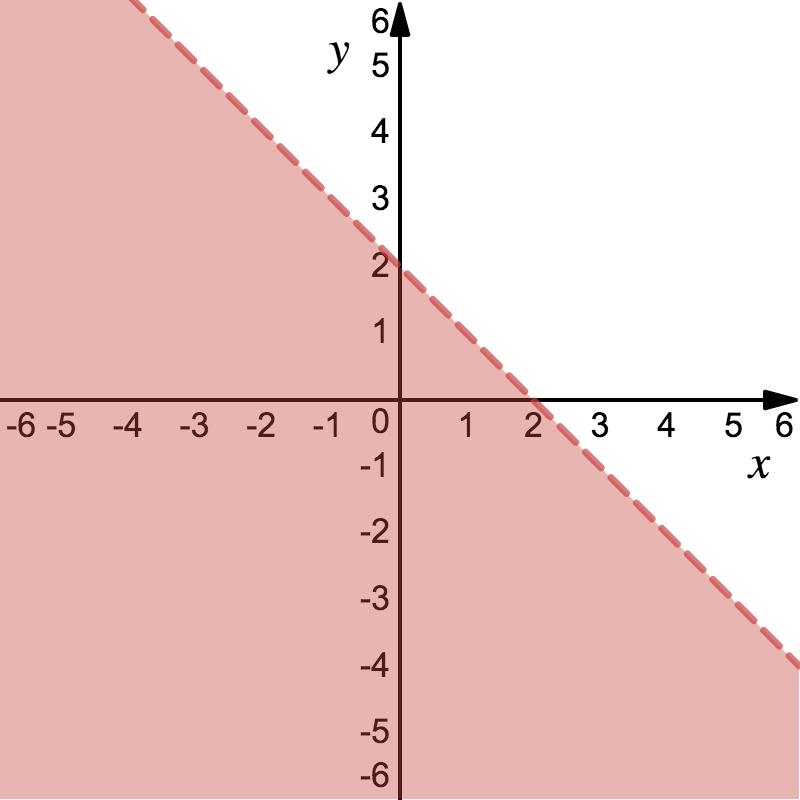
\includegraphics[width=4cm]{pics/pic6.png}
 \centering
  \caption{The graph of $x+y<2$.}
  \label{fig:fig_7}
\end{figure}
% 
Let's consider the second given inequality. Its boundary lines are $x=-2$ and $x=1$. The line of $x=1$ is not included. Because $x$ is between these two vertical lines, we shade the region between them. We must intersect this region with the red region in Figure \ref{fig:fig_7}. The resulting region is shown in purple.
% 
\begin{figure}[H]
 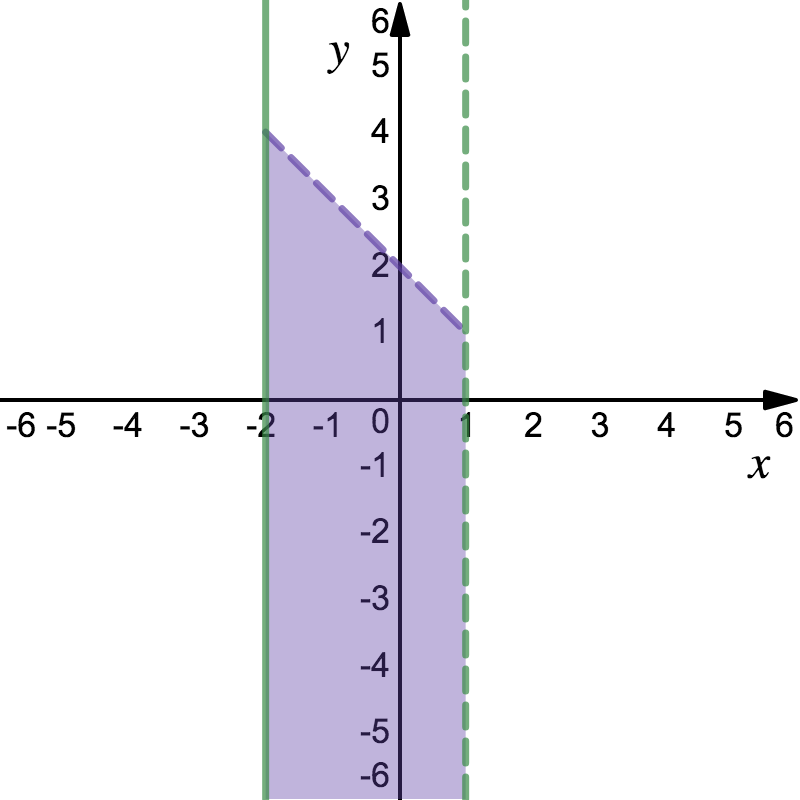
\includegraphics[width=5cm]{pics/pic7.png}
 \centering
  \caption{The graph of $x+y<2$ and $-2\leq x <1$.}
  \label{fig:fig_8}
\end{figure}
% 
Finally, let's consider the last given inequality, $y>-3$. Its boundary line is $y=-3$, which graphs as a horizontal line. Because of the greater than symbol in $y>-3$, the graph consists of the half-plane above the line $y=-3$. We must intersect this half-plane with the region in Figure \ref{fig:fig_8}. The resulting is shown in blue shading in Figure \ref{fig:fig_9}.
% 
\begin{figure}[H]
 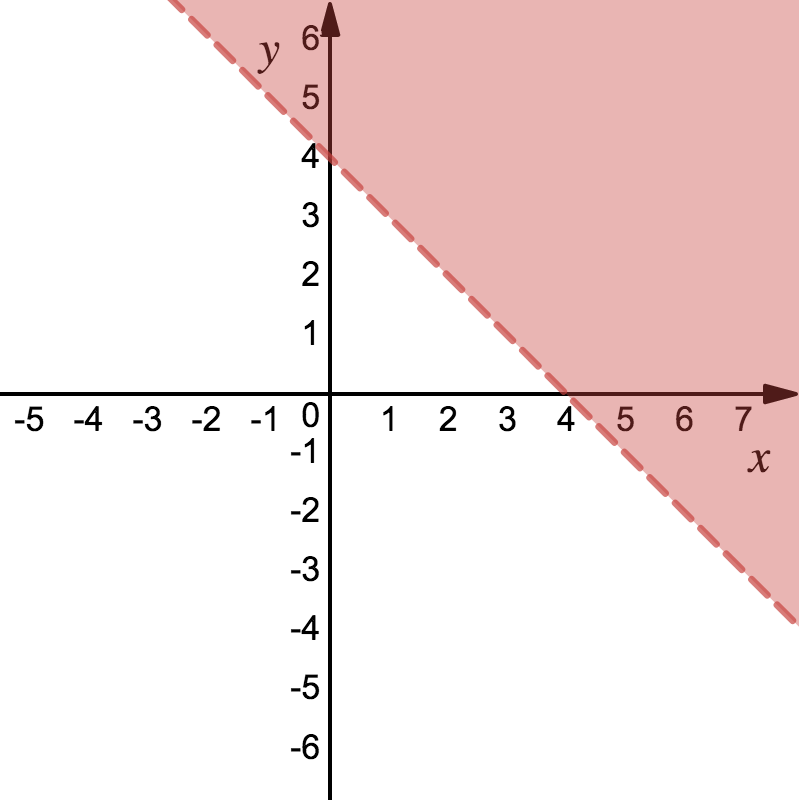
\includegraphics[width=5cm]{pics/pic3.png}
 \centering
  \caption{The graph of $x+y<2$, $-2\leq x <1$ and $y>-3$.}
  \label{fig:fig_9}
\end{figure}
% ==============








